\chapter{The Good Citizen}

These notes follow Michael Sandel's tenth lecture in the Justice course, curated here by LazyingArt LLC. We begin with Aristotle's break from Kant and Rawls, then follow the lecture through flutes, politics, civic virtue, the Casey Martin golf-cart case, and finally the objection that teleology leaves too little room for freedom. The order matters: each example is introduced not as an ornament but as the next test of the same claim, namely that arguments about justice cannot avoid arguments about the purpose of the practice at issue.

\section{From Rawls and Kant to Aristotle}

Sandel begins by marking a sharp contrast. Modern theories of justice often try to detach rights from moral desert and virtue. Aristotle does the opposite. On his view, justice asks what people deserve, and that question cannot be answered until we know what kind of activity or institution we are dealing with.

\begin{equation}
\text{justice}=\text{giving people what they deserve}
\end{equation}

This opening formula is compact, but it is not yet self-interpreting. To say that justice gives people what they deserve is not enough unless we can say what feature of a person is relevant in the case at hand. Sandel therefore immediately turns the lecture from a slogan into a method.

\begin{definition}
A teleological account of justice asks what a practice, institution, or good is for before deciding how it should be distributed. The purpose, or telos, fixes the relevant standard of merit.
\end{definition}

The point is not that every question of justice has the same answer. The point is that every such question requires the same kind of inquiry. We do not begin by asking who wants the good, or who can pay for it, or even who is in formal need of it. We begin by asking what the good is for.

\subsection{Question \& Answer}

Why is bare equality not enough?

Because the claim that equal things should go to equal persons still leaves open the decisive question. Equal with respect to what? Aristotle's answer, as Sandel presents it, is that the missing criterion comes from the nature of the thing distributed.

\begin{align}
\text{equal things} &\Longrightarrow \text{equal persons},\\
\text{equal in what respect?} &\Longrightarrow \text{look to the telos of the thing distributed}.
\end{align}

Once we see this, the lecture acquires its basic motion. Equality is not rejected, but interpreted. It is filled out by a prior account of purpose.

\section{Flutes, Telos, and the Honorific Turn}

Sandel does not remain at the abstract level for long. He turns at once to Aristotle's example of flutes, because it gives us a worked model of teleological reasoning before the lecture enters the more difficult terrain of politics and law. The question is simple: who should get the best flutes? Aristotle's answer is equally simple: the best flute players.

\paragraph{A worked Aristotelian example.}

We can write the structure of the example in a deliberately explicit way:

\begin{align}
\text{thing distributed} &= \text{flutes},\\
\text{telos} &= \text{good flute playing},\\
\text{relevant excellence} &= \text{excellence in flute playing},\\
\text{just recipient} &= \text{best flute players}.
\end{align}

This is more than a tidy example. It gives the lecture its first formal spine. We begin with the thing being distributed, identify its purpose, read off the excellence appropriate to that purpose, and only then decide who deserves the good.

\subsection{Question \& Answer}

Why should the best flutes go to the best flute players?

The answer is not merely that this arrangement produces more beautiful music, though Aristotle would not deny that. Sandel emphasizes a stronger point: the distribution itself expresses a judgment of worth. To give the best flutes to the best players is to honor the excellence of flute playing.

\begin{equation}
\text{rewarding the great flute player}
\Longleftrightarrow
\text{honoring the excellence of flute playing}
\end{equation}

This is the first moment at which Sandel makes explicit what will become one of the governing motifs of the lecture. Distributive questions are not only about who gets what. They are also about what qualities and excellences are recognized.

\begin{equation}
\text{debates about telos}
\Longrightarrow
\text{debates about honor}
\end{equation}

We can compress the pattern Sandel has in mind in the following schematic:

\begin{figure}
\centering
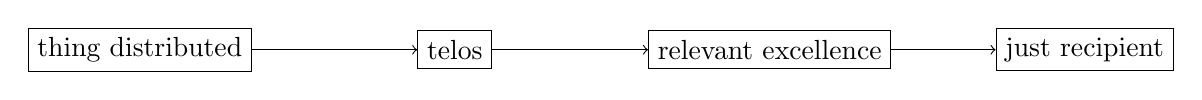
\begin{tikzpicture}
\node (a) [draw, rectangle] at (0,0) {thing distributed};
\node (b) [draw, rectangle] at (4,0) {telos};
\node (c) [draw, rectangle] at (8,0) {relevant excellence};
\node (d) [draw, rectangle] at (12,0) {just recipient};
\draw[->] (a) -- (b);
\draw[->] (b) -- (c);
\draw[->] (c) -- (d);
\end{tikzpicture}
\end{figure}

The lecture now widens its scope. Sandel says it is not easy to dispense with teleological reasoning in ethics and politics. To show why, he turns to two larger examples: politics and golf.

\section{Politics as the Distribution of Offices and Honors}

At this point Sandel changes not the method but the scale. Contemporary discussions of distributive justice usually concern income, wealth, and opportunity. Aristotle, by contrast, is concerned above all with offices, citizenship, authority, and rule.

\begin{align}
\text{modern distributive justice}
&\approx
\text{income}+\text{wealth}+\text{opportunity},\\
\text{Aristotelian distributive justice}
&\approx
\text{offices}+\text{honors}+\text{political rule}.
\end{align}

That change in subject matter is decisive. Once politics is understood as a matter of rule and citizenship, the question becomes: what is politics for? Only then can we ask who should rule.

Sandel's summary of Aristotle is blunt. Politics is not chiefly about securing private interests, protecting exchange, or preventing mutual injury. Its end is the good life.

\begin{align}
\text{telos of politics}
&=
\text{forming character}
+\text{cultivating virtue}
+\text{good life},\\
\text{mere life},\ \text{economic exchange},\ \text{security}
&\neq
\text{end of the polis},\\
\text{end of the polis}
&=
\text{good life}.
\end{align}

Here the lecture pauses over the modern objection. One can already hear the Kantian and Rawlsian reply: politics should not make us good; it should leave us free to choose our own ends. Sandel does not suppress that worry. He stages it at once, because it is precisely what makes Aristotle controversial.

\subsection{Question \& Answer}

If politics is for the good life, who should rule?

Sandel's Aristotelian answer is that political authority should go in greater measure to those who contribute most to the end of political association. If the polis aims at the good life, the standard of political distribution must be contribution to that aim.

We can write the argument in a compact derivational form:

\begin{align}
\text{telos of politics}
&\Longrightarrow
\text{criterion for distributing political authority},\\
\text{criterion for distributing political authority}
&=
\text{contribution to the good life of the polis},\\
\text{those who contribute most to the good life of the polis}
&\Longrightarrow
\text{greater share in rule and honor}.
\end{align}

This is not, in Sandel's telling, merely a disguised consequentialism. It is true that better rulers may produce better outcomes. But Aristotle's view is stronger than that. Politics itself is partly an institution for honoring civic excellence. Rule is not only an instrument; it is also a recognition.

\section{Why Political Life Matters to Human Flourishing}

Sandel now asks the question that naturally arises from the previous section. Why should participation in politics be essential to living well at all? Why can a person not lead a perfectly decent and moral life outside politics?

He says Aristotle gives two answers. The first comes from the Politics. Human beings are by nature political animals, and this is tied to language. We fully realize our nature only when we deliberate with one another about the just and the unjust.

\begin{align}
\text{human beings by nature}
&\Longrightarrow
\text{polis},\\
\text{isolated human being}
&\Longrightarrow
\text{beast or god}.
\end{align}

The point is not that the political community is temporally prior to the individual, but that it is prior in purpose. Outside the polis, the specifically human capacity for reasoned speech about right and wrong cannot be fully exercised.

The second answer comes from the Nicomachean Ethics, and it deepens the first. Happiness is not a feeling, and not the maximization of pleasure over pain. It is a kind of activity.

\begin{equation}
\text{happiness}
=
\text{activity of the soul in accordance with virtue}
\end{equation}

This formula does major work in the lecture. If happiness is activity in accordance with virtue, then a good political order cannot be indifferent to character. It must cultivate the conditions under which virtue can be formed.

Sandel then adds the practical point. Virtue is not learned by memorizing moral rules. It is acquired by practice, by doing, by developing the ability to discern particulars.

\begin{align}
\text{virtue} &\neq \text{book learning only},\\
\text{virtue} &\sim \text{practice},\\
\text{practice} &\Longrightarrow \text{discerning particulars}.
\end{align}

This is why the lecture lingers over examples that might otherwise seem expendable: flute playing, cooking, joke telling. We cannot become excellent in these activities by absorbing a rulebook and stopping there. We must acquire judgment in concrete situations. Aristotle, as Sandel presents him, thinks virtue is learned in the same way.

\subsection{Question \& Answer}

Why can we not live a fully good life outside politics?

Because the life of virtue requires more than private intention. It requires habits, practices, and the shared exercise of judgment with others. Sandel's two-step answer can be written as follows:

\begin{enumerate}
\item We realize our human nature through language and deliberation.
\item Deliberation about justice and the good is a political practice.
\item Happiness consists in activity in accordance with virtue.
\item Virtue is acquired by practice, not by precept alone.
\item Therefore the polis is not a mere shelter for private lives; it is one of the settings in which the human good is formed.
\end{enumerate}

This returns us to politics as a distributive question. If civic virtue is the relevant excellence, then those who possess it to the highest degree, Sandel's example is Pericles, deserve the greatest measure of offices and honors.

\begin{equation}
\text{civic virtue}
\approx
\text{deliberating among equals}
\end{equation}

\begin{equation}
\text{Pericles / greatest civic virtue}
\Longrightarrow
\text{greatest measure of offices and honors}
\end{equation}

And now the honorific dimension comes fully into view. Pericles should not rule only because he may govern well. He should also be singled out and honored as the citizen who most fully embodies the excellence politics exists to cultivate.

\section{Casey Martin and the Telos of Golf}

Having completed the politics example, Sandel turns to the contemporary controversy over Casey Martin. The move is not a digression. It is meant to show that even apparently modern rights disputes are driven by older questions about the nature and purpose of a practice.

Casey Martin is a gifted golfer with a circulatory condition that makes walking difficult and dangerous. He asks the PGA to permit him to use a golf cart in professional competition. The request is denied; the dispute reaches the Supreme Court. Sandel's question is moral as much as legal: should Martin have the right to use a cart?

\subsection{Question \& Answer}

Does Casey Martin have a right to use a golf cart, or does that depend on the purpose of golf?

Sandel's answer is unmistakably Aristotelian. The right cannot be settled first and the purpose asked later. Whether there is a right depends on whether walking is essential to the game.

\begin{align}
\text{rights claim in golf}
&\Longrightarrow
\text{depends on the telos of golf},\\
\text{walking essential to golf?}
&\Longrightarrow
\text{Casey Martin right to cart?}
\end{align}

This is why the classroom exchange matters. Some students argue that walking is intrinsic to golf, especially at the highest level. Others argue that Martin still bears pain and fatigue, and that the cart does not erase disadvantage but only mitigates it. Still others note that some tours already allow carts.

Sandel does not prematurely collapse these disagreements. He uses them to make a point about method. Even a dispute that presents itself as a matter of rights forces us to ask what golf is. Is it a game whose essential action is hitting the ball with the club? Or is walking, fatigue, and exertion part of the athletic whole?

The Supreme Court majority, as Sandel reports it, leans toward the first answer. Justice Scalia, in dissent, rejects the entire teleological frame. Courts, he argues, should not decide the essential nature of a game; games have no telos beyond amusement.

\begin{equation}
\text{game}=\text{mere amusement}
\end{equation}

Sandel explicitly identifies this as an anti-Aristotelian position. For Aristotle, a dispute over the rights internal to a practice can force us into a dispute over the purpose of that practice. Scalia denies that there is any such purpose to discover.

\section{The Recap Seam: Fairness and the Honor of Sport}

The lecture later returns to the golf case across a clear seam: when we ended last time, Sandel says, we were talking about Casey Martin's right to a cart. That reset matters. The argument is not merely repeated; it is sharpened.

The sharpening comes through Jenny's proposal. Why not make carts available to everyone? If the complaint is unfair advantage, let every golfer choose. This is a natural liberal solution: neutralize the asymmetry and leave the rest to preference.

\subsection{Question \& Answer}

Would allowing everyone to use a cart solve the fairness problem, or would it change the game?

The classroom exchange shows why Sandel thinks the issue is deeper than fairness narrowly understood. Da replies with the flippers analogy: if everyone may use flippers in swimming, we may equalize access to an aid while transforming the sport itself. Jenny responds that excluding a passionate and highly capable golfer may itself betray the spirit of the game. Michael insists that the PGA is the pinnacle and that its standards define entry.

What emerges is Sandel's second Aristotelian moral. The Martin case is not only about rights and not only about fairness. It is also about honor.

\begin{equation}
\text{golf controversy}
\Longrightarrow
\text{teleological dispute}+\text{honorific dispute}
\end{equation}

Why do elite golfers care so much? Sandel's answer is pointed and memorable: professional golfers are sensitive about whether their sport is really a sport. If everyone rides in a cart, golf may look less like an athletic competition and more like a game of skill. What is at stake, then, is not only the rulebook but the kind of excellence golf publicly honors.

We can write the lecture's compression of this point as follows:

\begin{equation}
\text{sport as practice}
\Longrightarrow
\text{calls forth and honors certain excellences}
\end{equation}

This is where Sandel answers Scalia most directly. Sports are not merely for amusement. Real sports are also for appreciation. They are practices that make intelligible disputes over which features are essential, precisely because those features help determine what excellence the practice prizes. If golf honors athletic excellence rather than mere hand-eye skill, then walking, fatigue, and exertion may be central rather than peripheral.

So the lecture's structure becomes visible again. Telos explains rights, and telos also explains honor. The case of golf is a contemporary version of the lesson already learned from flutes and politics.

\section{Freedom, Slavery, and the Objection to Teleology}

Only after flutes, politics, and golf are in place does Sandel turn to the major objection. If justice is a matter of fit between persons and roles, what happens to freedom? What room is left for my right to choose my ends for myself?

\begin{equation}
\text{justice as fit}
=
\text{fitting persons with virtues/excellences to appropriate roles}
\end{equation}

\begin{equation}
\text{teleology}
\Longrightarrow
\text{freedom objection}
\end{equation}

Sandel does not dismiss the objection. He intensifies it by turning to Aristotle's defense of slavery, the most troubling application of the doctrine of fit. Aristotle's own account, as Sandel reconstructs it, imposes two conditions: slavery must be necessary for the functioning of the polis, and it must be fitting by nature for those enslaved.

\begin{align}
\text{slavery just}
&\Longrightarrow
\text{necessary} \land \text{fitting by nature},\\
\text{actual Athenian slavery}
&\not\Longrightarrow
\text{natural fit},\\
\text{coercion}
&\Longrightarrow
\text{evidence of misfit / not natural}.
\end{align}

The lecture is careful here. Sandel does not say that Aristotle has no internal standards. On the contrary, he uses Aristotle's own standards against Aristotle's own application. Many actual slaves in Athens were captives of war, enslaved by bad luck rather than by any alleged natural fitness for servitude. If so, then the institution as practiced fails the criterion of fit.

This matters because Sandel wants to show two things at once. First, Aristotle's defense of slavery is deplorable. Second, the failure of that defense does not by itself refute the entire teleological structure, because the application may be faulty even if the general form of the argument is intelligible.

\subsection{Question \& Answer}

If justice depends on telos and fit, what room is left for freedom and individual choice?

The students' objections make the issue vivid. If I am supposedly well suited to some role, must I occupy it? If I disagree with the community about the ends of our shared life, how can justice be grounded in any single account of the good? Sandel lets these objections stand in full force, because they are precisely what lead back to Kant and Rawls.

Patrick's objection is that teleological reasoning may never yield agreement in a pluralist society. Mary Kate's objection is that even a fitting role may not be a chosen role. Sandel treats both as serious. Modern political theory, he says, often begins from this very worry and concludes that justice and rights must not rest on any controversial conception of the good.

The lecture therefore ends not with a settled verdict but with a pair of questions that will govern the next confrontation between Aristotle, Kant, and Rawls:

\begin{equation}
\text{right prior to good?}
\qquad
\text{chooser of ends vs discoverer of nature}
\end{equation}

This is the right place for the lecture to stop. We have seen why Aristotle thinks justice cannot avoid teleology, and we have also seen why liberal theory is driven to resist that conclusion.

\section{Summary}

The lecture begins with Aristotle's refusal to detach justice from desert and virtue, and it develops that refusal through a sequence of examples of increasing difficulty. The flute case gives us the basic template: the telos of the thing distributed determines the relevant excellence and therefore the just recipient. Politics enlarges the template into a theory of citizenship, civic virtue, and the good life. The Casey Martin case shows that even modern rights disputes over accommodation and fairness depend on arguments about the purpose of a practice and the excellences it honors. Finally, the discussion of slavery and freedom brings us to the limit-point of teleological justice. Sandel leaves us there deliberately, with the deepest question still open: whether justice must be anchored in an account of the good, or whether freedom requires that the right stand prior to it.